\section{Обзор существующих решений}
\label{sec:Chapter4} \index{Chapter4}

%В данной главе необходимо провести анализ существующих моделей. Аргументировать выбор тех или иных моделей, методов. Подготовить теоретическую базу перед экспериментов.


\subsection{Обзор моделей для распознавания ключевых точек}
\label{sec:Chapter4_PE}

В данном разделе будут рассмотрены несколько моделей распознавания ключевых точек на теле человека. Некоторые из них довольно старые, но показывают неплохие результаты. Большинство же представлены не более 5 лет назад и являются лидерами направления на сегодняшний день.

\subsubsection*{DeepPose}

Данный представитель является самым старым решением из данной выборки и, одновременно, один из самых первых в целом. Статья "DeepPose: Human Pose Estimation via Deep Neural Networks"   \cite{DeepPose} была представлена исследователями из GOOGLE на конференции CVPR в 2014 году.

Исследователи разработали модель, представляющую сосбой каскад из DNN-регрессоров для локализации ключевых точек. Так как на тот момент не было выпущено общепринятых топологий, то в роли ключевых точек выступали суставы тела, а поза кодировалась их координатами, нормализованными на размер изображения.

\begin{figure}[h]
	\centering
	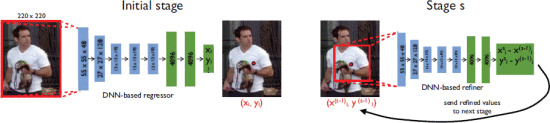
\includegraphics[width=\textwidth]{./images/DeepPose}
	\caption{Архитектура сети DeepPose. \cite{DeepPose}}
	\label{fig:dp_architecture}
\end{figure}

Работа модели делилась на два этапа, которые схематически показаны на \autoref{fig:dp_architecture}. На первом производилась локализация точки. Далее результаты переходили на второй этап, где пропускались через каскад из DNN, который производил уточнение предсказания. В результате получался отосительно точный результат, который можно было использовать для дальнейших исследований.


\subsubsection*{OpenPose}

OpenPose - это проект от лаборатории перцептивных вычислений университета Карнеги-Меллона в США. Проект включает в себя несколько моделей распознавания ключевых точек: на лице, руках, теле и различные их комбинации. Количество распознаваемых моделями точек доходит до 135 на одном человеке, а модель может распознавать сразу несколько человек на одном кадре. Скорость работы модели позволет использовать ее для распознавания видео в реальном времени через веб-камеру. К сожалению, основной репозиторий проекта не поддерживается с ноября 2020 года.

\begin{figure}[h]
	\centering
	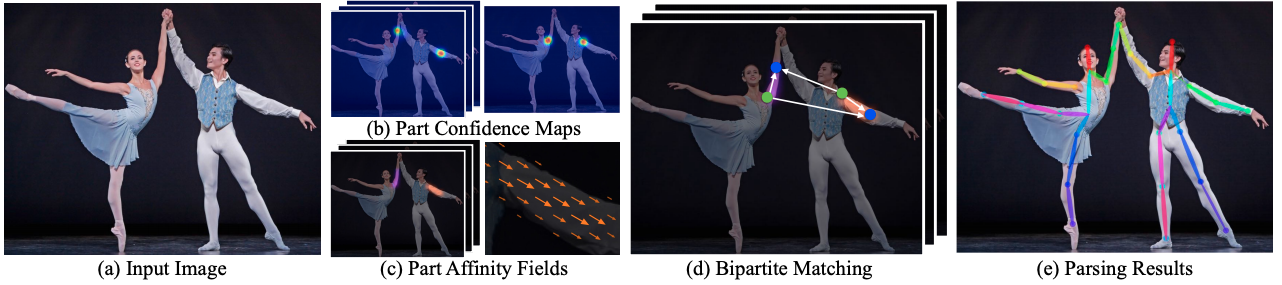
\includegraphics[width=\textwidth]{./images/OpenPose/structure}
	\caption{Последовательность распознавания ключевых точек моделью OpenPose. \cite{OpenPose}}
	\label{fig:op_structure}
\end{figure}

На данный момент обратимся к модели, резльтаты которой описываются тополгией из 25 точек. Данная модель одна из немногих в представленном обзоре, которая использует подход снизу вверх. Это достигается за счет использования двухступенчатой архитектуры нейросети (см \autoref{fig:op_structure}). 
 
В рамках первого этапа (вторая колонка на \autoref{fig:op_structure}) нейросетью предсказываются такие сущности, как карта достоверности обнаружения точки и карта двумарных векторных полей ориентации конечностей (англ. Part Affinity Fields или PAF). Изначально предсказание сущностей выполнялось паралельно, но взаимный анализ результатов предсказаний позволил увидеть возможность интуитивно предсказывать карты достоверности на основе PAFs. Это позволило значительно ускорить работу алгоритма.

Вторым этапом (треья колонка на \autoref{fig:op_structure}) происходит сопоставления точек и конечностей отдельным людям. Для увеличения точности и уменьшения времени построения скелетов используются графы соответсвия, которые позволяют создать целостные и непротиворечивые представления поз людей на изображении.

\subsubsection*{HRNet}

Решение на основе архитектуры HRNet, опубликованной в 2019 году, является одним из первых, представленных в проекте MMPose. Оно использует подход сверху-вниз, в котором для детекции используется модель из проекта MMDetection.

\begin{figure}[h]
	\centering
	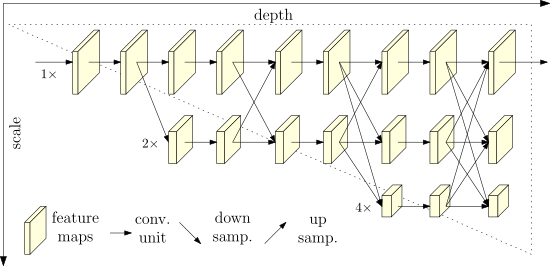
\includegraphics[width=.9\textwidth]{./images/hrnet_architecture}
	\caption{Архитектура модели HrNet. \cite{hrnet}}
	\label{fig:hrnet_architecture}
\end{figure}

Особенность архитекртуры HRNet является возможность поддерживать высокое разрешение изобажений на всех этапах обработки, что позволяет достичь высокой точности и детальности предсказаний. Достигается это за счет параллельного использования нескольких ветвей с разным разрешением и постоянного обмена информацией между ними (см. \autoref{fig:hrnet_architecture}).

Все начинается с уровня слоев высокого разрешения, к которому паралельно добавляются слои с пониженным разрешением. Периодически между ветвями происходит обмен  информацией с помощью fusion module. Этот процесс обеспечивает сбалансированное и детализированное представление на разных уровнях разрешения, что приводит к улучшению точности получаемого результата.

\subsubsection*{BlazePose}

\begin{figure}[b]
	\centering
	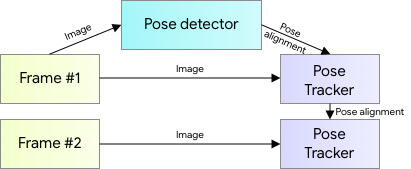
\includegraphics[width=.8\textwidth]{./images/BlazePose/Model_structure.jpg}
	\caption{Структура модели BlazePose для работы в реальном времени. \cite{BlazePose}}
	\label{fig:mp_model_structure}
\end{figure}

Архитектура нейросети BlazePose разработана в 2020 году ислледователями от GoogleResearch и известна своим использованием в работах проекта MediaPipe \cite{BlazePose, mediapipe}. Она предназначена для бытрого и точного распознавания ключевых точек тела в реальном времени, даже на мобильных устройствах и в условиях ограниченных вычислительных ресурсов. Расширенная до 33 точек топология модели помогает использовать нейросеть в разнообразных сопртивных приложениях, таких как фитнес-трекеры и анализаторы асан йоги.

BlazePose использует top-down подход оценки позы, который оптимизирован для работы с видеопотоками. Схематично, структура нейросети представлена на \autoref{fig:mp_model_structure}. На первом этапе необходимо найти человека на входном изображении, чем и занимается PoseDetector. Но он вызывается только для первого кадра и возвращает не только координаты облати с человеком, а информацию об интересующей нас области (region of interest или ROI). Именно ROI дает возможность не звызывать каждый раз детектор, так как она изменяется на втором этапе работы сети и передается сразу для использования в Pose Tracker следующего кадра.

\begin{figure}[h]
	\centering
	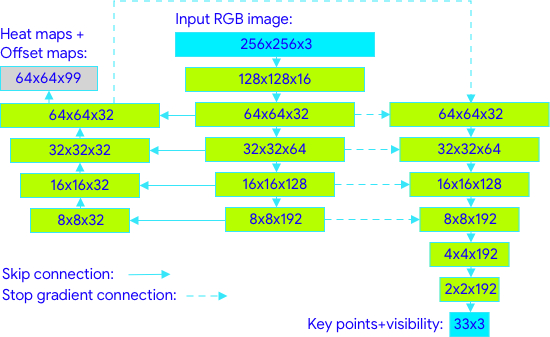
\includegraphics[width=.8\textwidth]{./images/BlazePose/architecture.jpg}
	\caption{Архитектура Pose Tracker. \cite{BlazePose}}
	\label{fig:mp_architecture}
\end{figure} 

Следующим шагом является распознавание КТ в заданной области интереса. Путем использования нескольких пирамидальных архитектур производится комбинированны анализ тепловой карты и данных о смещении (см. \autoref{fig:mp_architecture}).

\subsubsection*{ViTPose}

ViTPose - это модель для распознавания ключевых точек, которая была представлена в 2022 году командой исследователей из университета Сиднея \cite{vitpose}. В ее основе используется архитектура трансформера, которые изначально были разработаны для обработки последовательностей в задачах обработки естественного языка, адаптированного для задач компьютерного зрения (англ. Vision Transformer или ViT) \cite{vit}. Данный подход продемонстрировал высокую эффективность и конкурентоспособность по сравнению с традиционными свёрточными нейронными сетями (CNN), что позволило область решений задачи оценки позы.

\begin{figure}[h]
	\centering
	\includegraphics[width=.9\textwidth]{./images/vitpose_structure}
	\caption{Структура VitPose (a). Блоск трансфрмера (b). Классический декодер (c). Простой декодер (d). Декодеры для нескольких наборов данных (e). \cite{vitpose}}
	\label{fig:vitpose_structure}
\end{figure}

Для создания анализируемой последовательности изображений разбивается на патчи рамером $16x16$. Они прогоняются через линейные слои нейросети для получения эмбеддинга, к которому дополнительно добавляется позиционный эмбеддинг, чтобы модель могла учитывать пространственное расположение блоков. И потом уже полученная цепочка векторов передается на вход магистральной части нейронной сети. Используя механизмы самовнимания (англ. self-attention), которые помогают использовать различные взаимосвязи между частями изображения, backbone возвращает признаковое описание изображения.

Для извлечения признаков и локализации ключевых точек из результатов магистральной части испоьзуется два типа декодеров. Классический декодер использует несколько блоков для повышения дискретизации тепловой карты ключевых точек, а для локализации координат используется сверточный слой в качестве выходного слоя. Другой декодер, называемый в работе <<простым>> \cite{vitpose}, использует один слой билинейной интерполяции для повышения детализации результатов, а для получения тепловых карт используется функция активацции RELU. Предсказателем также выступает сверточный слой.


\subsubsection*{Simcc}
\label{subsec:simcc}

Локализация ключевых точек на основе анализа тепловых карт достоверности является весь распространенным подходом в задаче оценки позы. Но даже этот подход имеет некоторые недостатки: плохие результаты на изображениях низкого разрешения, вычислительно тяжелые слои повышения дискретизации тепловых карт и дополнительная постобработка для уменьшения ошибок квантования. Чтобы избежать их исследователями был разработан алгоритм Simple Coordinate Classification или SimCC \cite{simcc}, который предлагает новый подход к оценке поз человека с помощью классификации отдельно горизонтальных и вертикальных координат. Схематическое описание алгоритма представлено на \autoref{fig:simcc_structure}.

\begin{figure}[h]
	\centering
	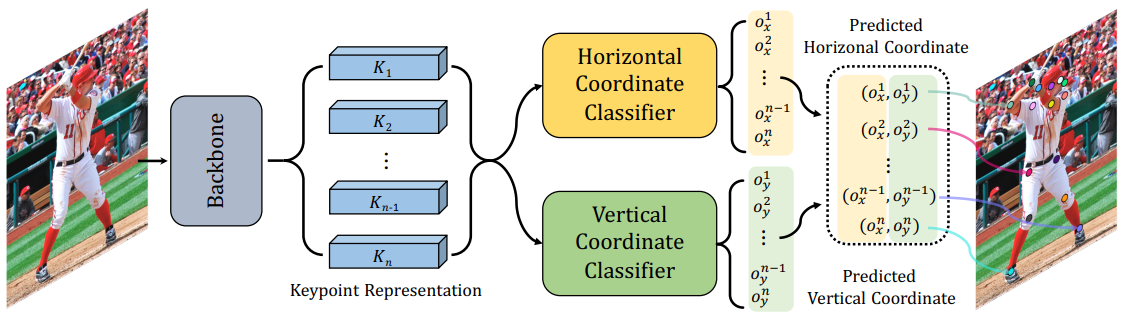
\includegraphics[width=\textwidth]{./images/simcc_structure}
	\caption{Структура SimCC \cite{simcc}}
	\label{fig:simcc_structure}
\end{figure}

Для извлечения признаков в данном алгоритме используется магистральная нейронная сеть, которой могут быть как сверточные нейронные сети, так и трансформеры. Она возвращает признаковое описание необходимого количества ключевых точек.

Для дальнейшего шага все координаты дискретезируются на более мелкие бины, чтобы избежать ошибок квантования. Далее классификатор выставляет метки всем бинам, причем делает это независимо для вертикального и горизонтального направления. А для обучения модели используется функция потерь на основе дивергенции Кульбака-Лейблера (англ. Kullback-Leibler divergence).

В итоге алгоритм показывает немного более лучшие результаты, в сравнение с решениями на основе анализа тепловых карт, но сильно уменьшает количество проводимых операций, чем значительно улучшает скорость работы модели.

\subsubsection*{YoloPose}

Yolo-Pose - это семество решений на основе архитектуры Yolo, которое представляет собой новаторский подход для одновременного обнаружения нескольких человек на фото и распознавания их скелета. Алгоритм был предъявлен публике в 2022 году исследователями из Техаса \cite{yolo_pose}. В своей статье они использовали архитектуру Yolo5, которая показывала хорошие результаты распознавания ключевых точек на датасете COCO. На сегодняшний день к семейству Yolo-Pose подтянули и других представителей популярной архитектуры, таких как Yolo8, YoloX и Yolo-NAS \cite{yolo8, yolox}.

\begin{figure}[h]
	\centering
	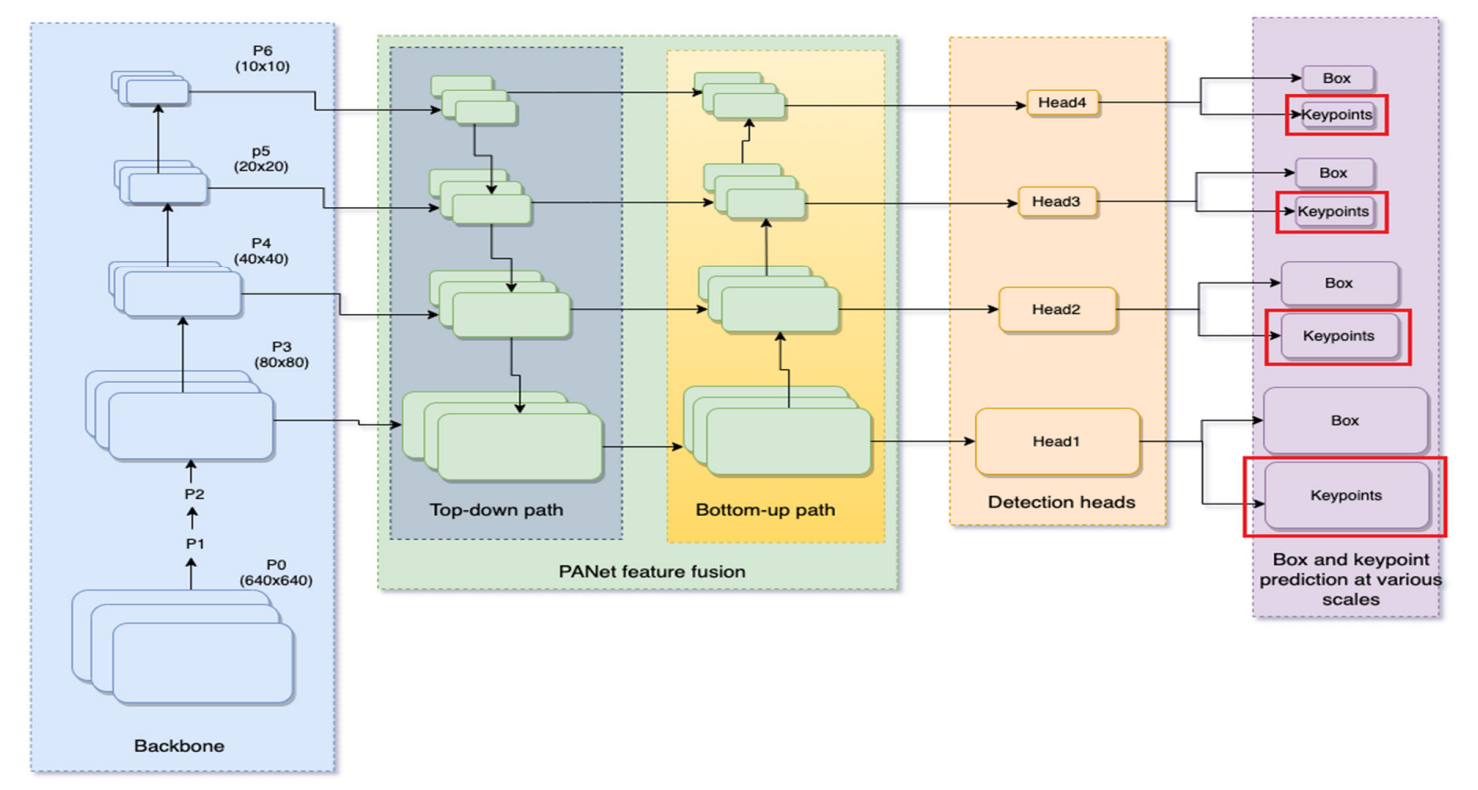
\includegraphics[width=\textwidth]{./images/yolo_pose}
	\caption{Архитектура Yolo-Pose на основе модели Yolo5. \cite{yolo_pose}}
	\label{fig:yolo_pose}
\end{figure}

Авторы решили пересмотреть использование различных подходов к распознаванию ключевых точек и совместили лучшее из обоих вариантов. Большинство подходов сверху-вниз используют тепловые карты для предсказания координат ключевых точек. Как уже было сказано в \autoref{subsec:simcc}, детализация тепловых карт занимает множество вычислительных ресурсов. А ещё производительность этих решений напрямую зависит от количества человек на изображении, так как все они распознаются по отдельности. В свою очередь подходы снизу-вверх имеют сложность при сопоставлении ключевых точек отдельным людям. В итоге получилось построить решение, которое производит поиск человека на фото, присваивает ему некоторую якорную точку (англ. anchor point), с которой в последвтии ассоциируются все ключевые точки и ограничивающая рамка. А разделение на две сущности: bbox и keypoints происходит на этапе обработки полученных признаков (head) и предсказания результатов.

Полученный алгоритм сквозного обучения не мог работать на существующих L1 метриках, поэтому исследователи оптимизировали метрику OKS для обучения моделей (о метрике рассказано в \autoref{sec:Chapter5}). Это дало возможность учитывать весовые коэфициенты точек и масштаб объекта при обучении.

Но у моделей этого семейства есть и минус. Это требования большого количества вычислительных ресурсов для обучения моделей. Что делает практически невозможным улучшение модели простым обывателем. 

\subsubsection*{RTMPose}

Из текущей подборки данная архитектура является самой молодой. Алгоритм создан в 2023 году и специально оптимизирован для распознавания поз нескольких человек в реальном времени, о чем говорит его название: <<RTMPose: Real-Time Multi-Person Pose Estimation>> \cite{rtmpose}. Он вобрал в себя лучшие методики последних лет и показывает очень хорошие результаты как в точности, так и в скорости инференса.

\begin{figure}[h]
	\centering
	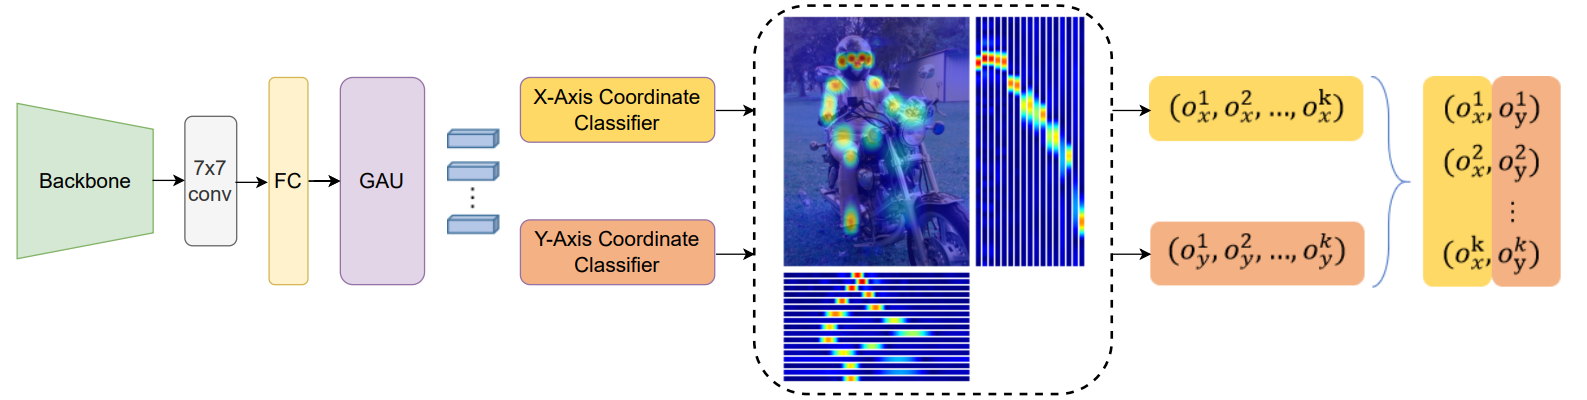
\includegraphics[width=\textwidth]{./images/rtmpose}
	\caption{Общая архитектура RTMPose. \cite{rtmpose}}
	\label{fig:rtmpose_architecture}
\end{figure}

RTMPose поддерживает top-down подход, поэтому для работы ему необходим детектор. В рамках проекта MMPose используется детектор RTMDet, разработанный в той же лаборатории \cite{mmpose, rtmdet}. Для ускорения работы нейросети на видеозаписях используется идея, предложенная в BlazePose \cite{BlazePose}: использование детектора только на первом кадре, при работе алгоритма вносить изменения в ROI и уже измененные прямоугольники передавать для следующего кадра без задействования дополнительной модели. Это позволяет получать более высокие показатели скорости работы в реальном времени.

Рассмотрим архитектуру нейронной сети, которая представлена на \autoref{fig:rtmpose_architecture}. Для извлечения признаков используется базовая нейронная сеть CSPNeXt, которая показывала хорошие результаты в задаче детекции объектов. Для выуживания координат из полученной карты признаков используют описанный ранее алгоритм SimCC \cite{simcc}. Таким образом с помощью классификаторов предсказываются отдельно горизонтальные и вертикальные координаты точек, что показывало 69.7 AP на датасете COCO. Однако и текущие результаты получилось улучшить.

Было замечено, что при увелчении размерности полученных признаков улучшается результат предсказания. Поэтому между магистральной сетью и классификаторами добавили полносвязный слой, который увеличивает размерность полученных представлений ключевых точек. Также после этого добавлен модель самовнимания, основанный на Gated Attention Unit
(GAU). Это изменение обеспечио более внимательное использование глобальой и локальной пространственной информации.

В итоге предложенный алгоритм достиг 75.8 AP на датасете COCO и скорости 90 кадров в секунду без использования графических ускорителей.


\subsection{Обзор методов доменной адаптации на неразмеченных данных}
\label{sec:Chapter4_DA}

%Опираясь на модели из предыдущей главы надо сделать анализ и выбрать только несколько методов, которые применимы к нашим требованиям и которые мы будем сравнивать между собой.

\subsubsection*{Progressive Unsupervised Learning}

Встречаясь с чем-то новым, люди могут несколько раз рассматривать, пробовать и анализировать новый предмет, прежде чем получат необходимые знания о нем. Похожую схему использует алгоритм прогрессивного обучения без учителя (англ. progressive unsupervised learning или PUL). Его концепция позволяет избавиться от необходимости аннотировать данные для дообучения нейронных сетей на них, тем самым позволяя моделям адаптироваться к новому домену. Первоначально модель была применена в задаче отслеживания объектов \cite{pul}, а позже использована в задаче повторной идентификации человка \cite{pul_person}.

\begin{figure}[h]
	\centering
	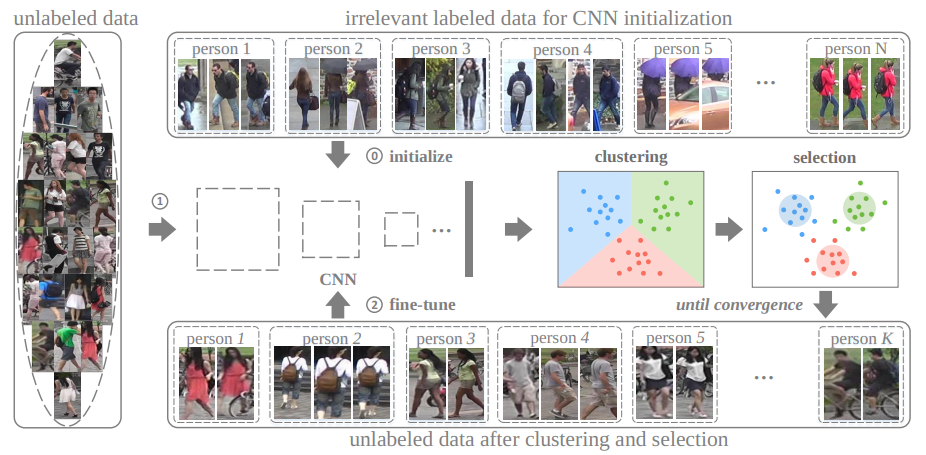
\includegraphics[width=.8\textwidth]{./images/pul}
	\caption{PUL \cite{pul_person}}
	\label{fig:pul}
\end{figure}

Основная концепция алгоритма, как метода unsupervidsed domain adaptation, состоит в отсутствии необходимости размечать данные, а адаптироваться к ним посредством итеративного обучения на псевдоразметке. Опишем действия, которые будут выполняться повторно.

\begin{enumerate}

\item \underline{Входные данные}\\
Для начала работы алгоритма необходимо иметь некоторое преварительно обученное состояние модели.

\item \underline{Псевдоразметка данных}\\ 
Неразмеченные данные прогоняются через модель для получения некоторых результатов. Из-за того, что модель имеет некоторую ошибку, текущие результаты называются псевдо-разметкой.

\item \underline{Фильтрация невалидных результатов}\\
Модель может значительно ошибаться в предсказании псевдо-разметки, поэтому необходимо обозначить некую функцию фильтрации шумных значений. Например, при применении PUL к задаче повторной идентификации \cite{pul_person}, была построена интересная функция фильтрации на основе кластеризации вектора признаков изображения и отбрасывания всех значений, значительно далеких от центра кластера.

\item \underline{Обучения модели}\\
Производится дообучение модели на полученных данных. Состояние модели после дообучения передается на вход следующей итерации алгоритма. 
\end{enumerate}

Маркерами для остановки итеративного, помимо заранее определенного количетсва итераций, процесса могут служить:
\begin{itemize}
\item Стабильность кластеров\\
Когда кластеры псевдоразмеченных данных стабилизируются и изменения в них между итерация становятся минимальными.
\item Устойчивость к шуму\\
Когда количество зашумленных данных становится минимальным или приемлемым.
\item Сходимость функции потерь\\
Если функция потерь, используемая для обучения модели, перестает значительно уменьшаться между итерацциями, то это указывает на сходимость модели.
\item Критерий качества результатов\\
Когда достигается определенное заранее выбранное значение метрики качества на целевых данных. Данный метод хорош при небольшом количестве размеченных данных на целевом домене.
\end{itemize}

\subsubsection*{Regressive Domain Adaptation}

Большинство современных алгоритмов доменной адаптации без учителя изначально созданы для применения в задачах классификации и могут не работать в задачах регрессии, например к задаче распознавания ключевых точек. Поэтому был предложен алгоритм регрессивной доменной адаптации (англ. Regressive Domain Adaptation или RegDA) \cite{regda}.  

\hfill \break

НАДО БУДЕТ ОСТАВИТЬ ТОЛЬКО ОДИН ИЗ СЛЕДУЮЩИХ МЕТОДОВ.

\subsubsection*{UDA PoseEstimation}

Адаптация от синтетических данных к реальным. Должно бтыь интересно описать. Не использовали, так как до сих пор мы не перешли в 3х мерное пространство.

\subsubsection*{POST}

Похожее на предыдущее

\subsubsection*{SFDA}

Похожее на предыдущее


\newpage
